\begin{figure}[!htbp]
    \centering
    % \begin{subfigure}[b]{0.49\textwidth}
    %     \centering
    %     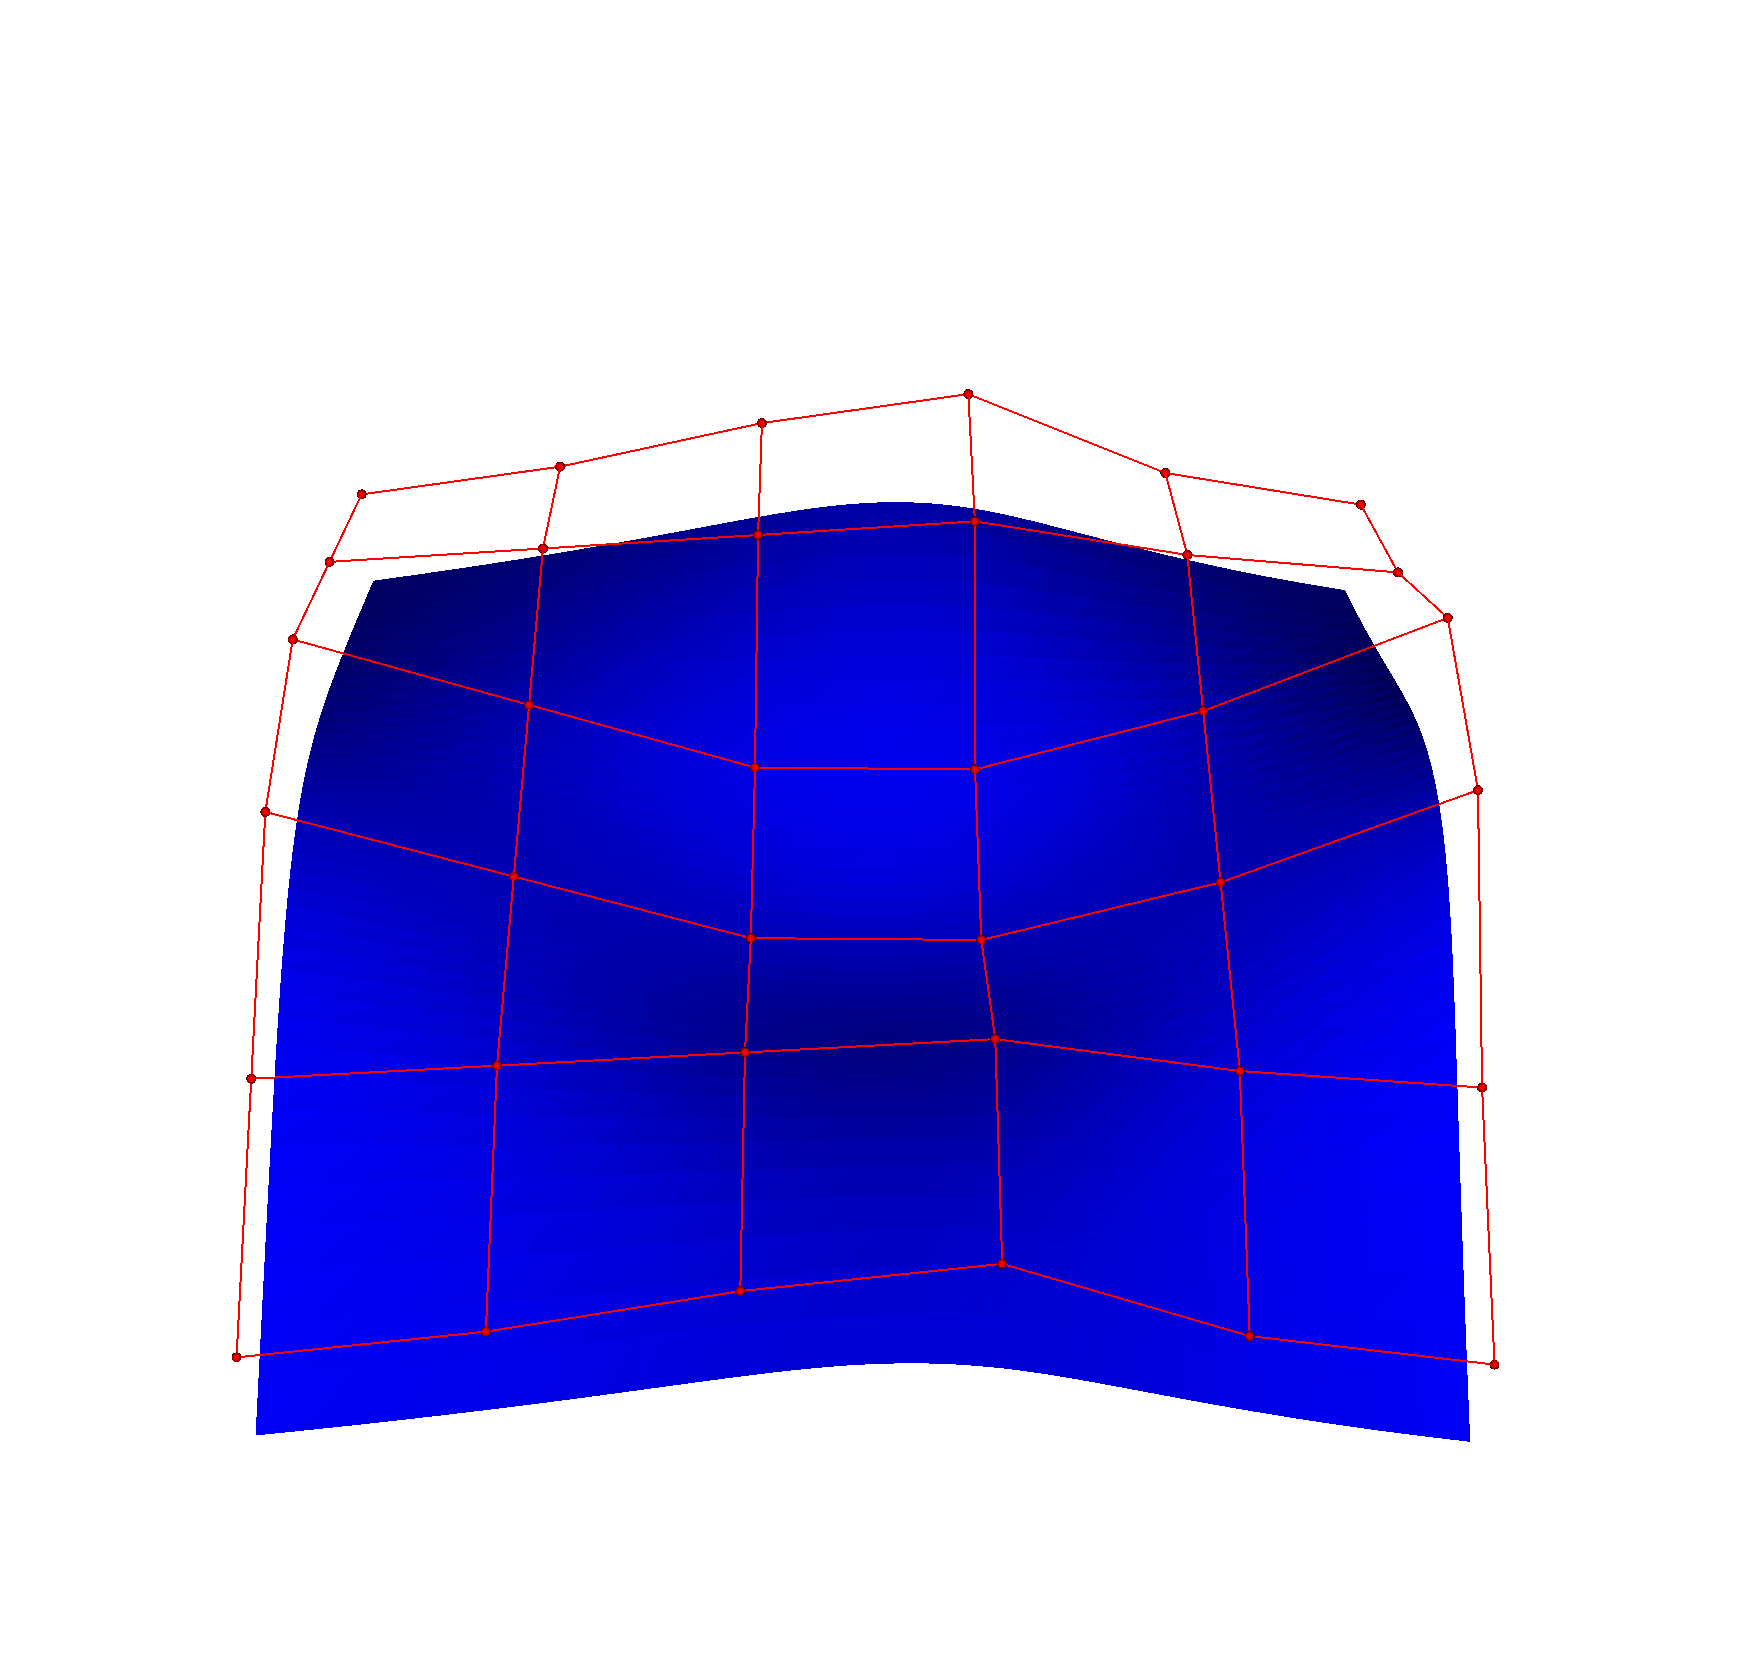
\includegraphics[height=\textwidth, trim=90 90 90 90, clip]{figures/registration/splines/spline2.png}
    % \end{subfigure}
    \begin{subfigure}[b]{0.49\textwidth}
        \centering
        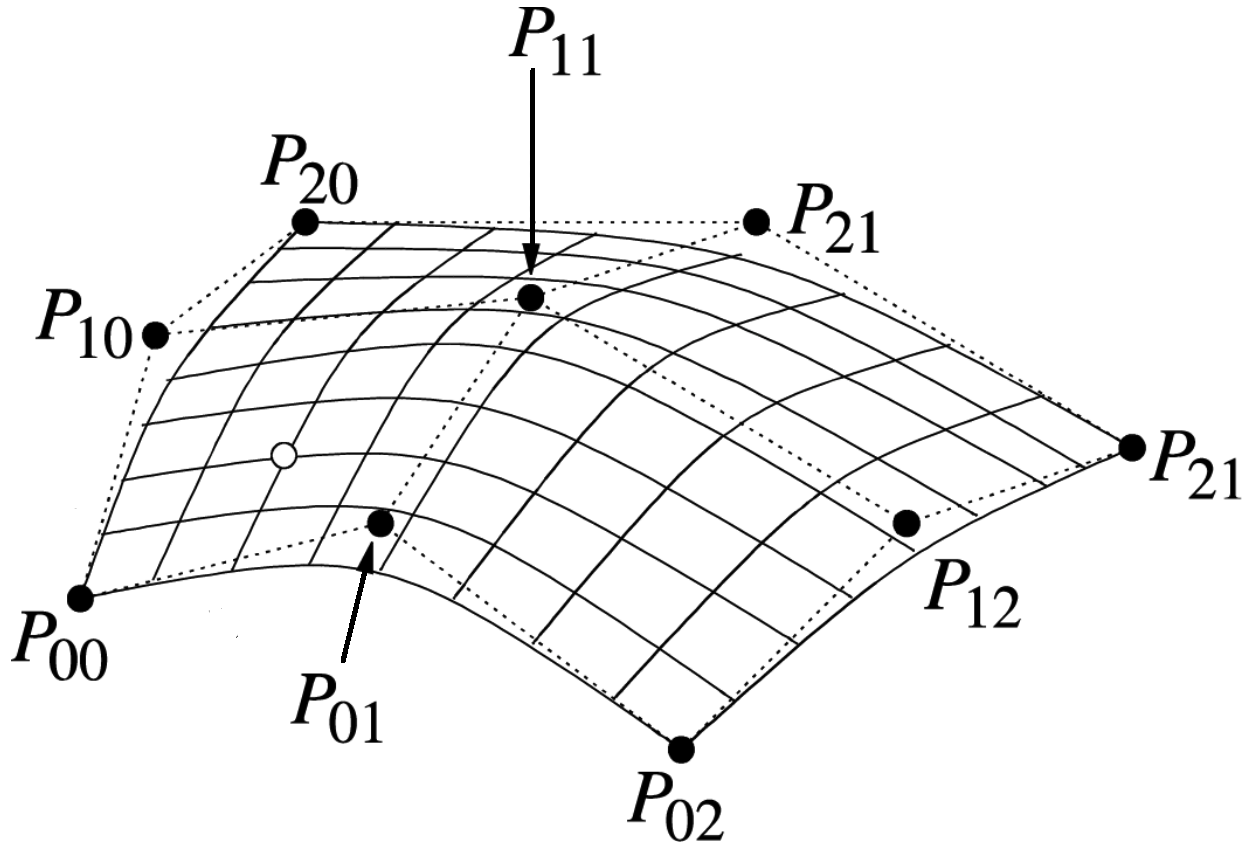
\includegraphics[height=.6\textwidth]{figures/registration/splines/spline5.png}
        \caption{Bicubic spline.}
        \label{fig:bicubicspline}
    \end{subfigure}
    \vskip\baselineskip

    % \begin{subfigure}[b]{0.49\textwidth}
    %     \centering
    %     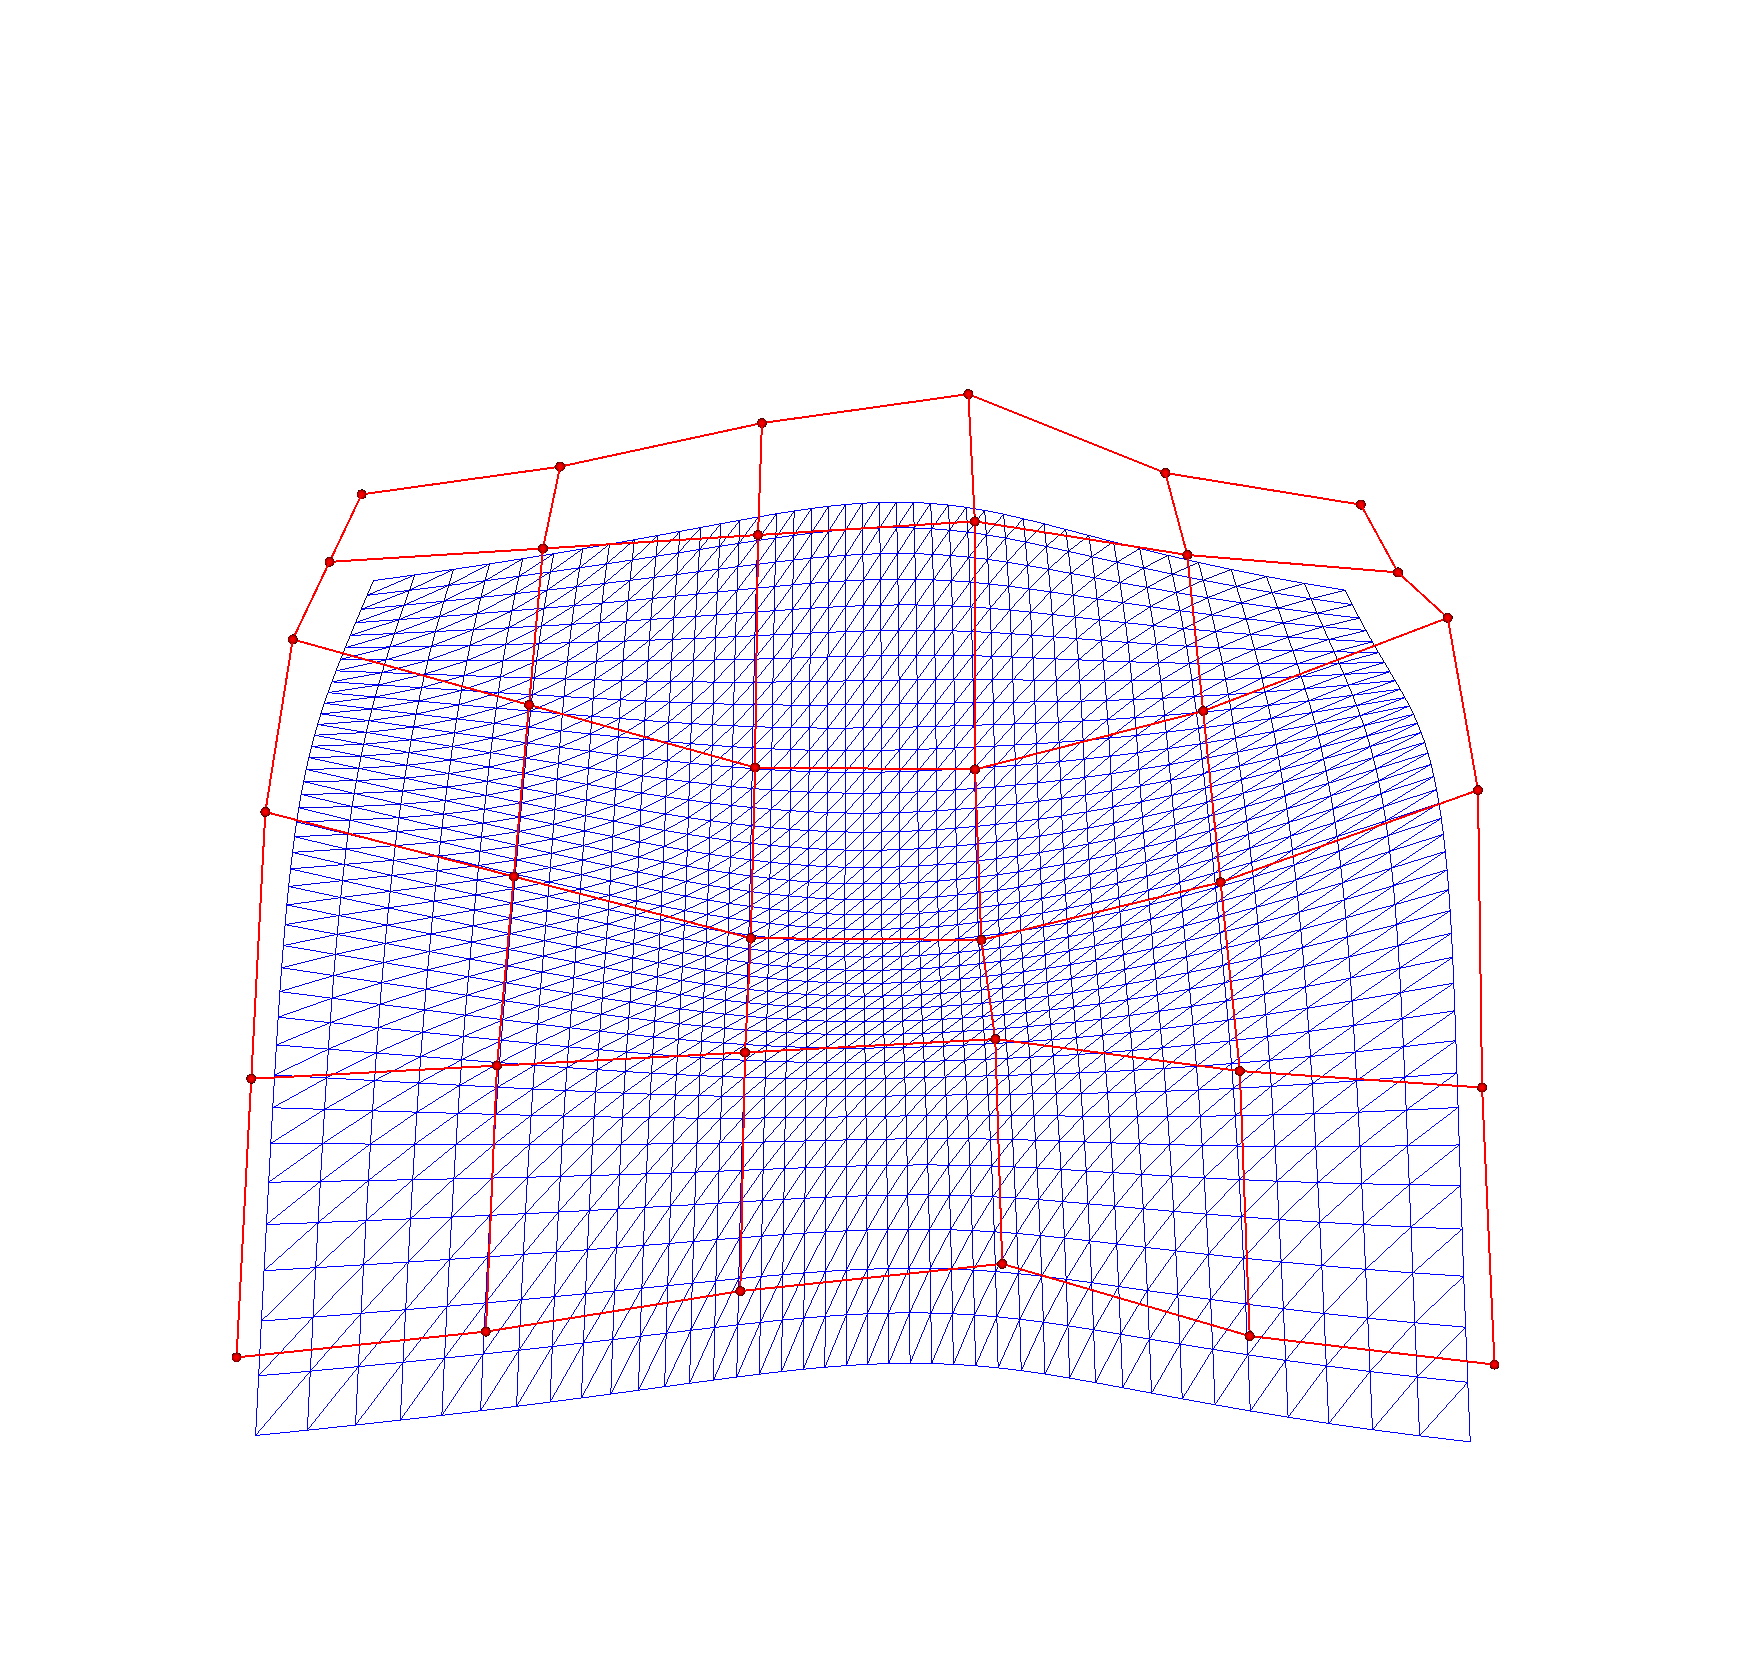
\includegraphics[height=\textwidth, trim=90 90 90 90, clip]{figures/registration/splines/spline3.png}
    % \end{subfigure}
    \caption{Splines with control points emphasized.}
    \label{fig:spline}
\end{figure}